\documentclass[12pt]{article}
\usepackage{graphicx}

\usepackage[section]{placeins}
\graphicspath{ {./img/} }
\usepackage[a4paper, total={6in, 9in}]{geometry}
\usepackage{hyperref}
\usepackage[utf8]{inputenc}
\usepackage[english]{babel}
\usepackage{fancyhdr}
\usepackage{chemformula}
\usepackage{xcolor}
\usepackage{float}
\usepackage{tabto}
\usepackage{subcaption}
\usepackage{tikz}
\usepackage[section]{placeins}
\usepackage{booktabs}
\usepackage{adjustbox}
\usepackage{array}
\usepackage{gensymb}
\usepackage[siunitx, RPvoltages]{circuitikz}
\usetikzlibrary{shapes, arrows}

% Figure Setup
\tikzstyle{boxes} = [rectangle, minimum width=2cm, minimum height=1cm, text centered, text
width=3cm, draw=black]

\tikzstyle{line} = [thick, -, >=stealth]
\tikzstyle{arrow} = [thick, ->, >=stealth]

\title{{\huge \textbf{ENEL420 Assignment 1}}\vspace{20pt}\\Digital Filtering of Additive Noise on an ECG Signal\vspace{24pt}}
\author{\large Joshua Hulbert (21385664)\\\vspace{12pt}\large Josiah Craw (35046080)}

\begin{document}
\maketitle
\thispagestyle{empty}

\newpage
\section*{Abstract}
\pagenumbering{roman}
An electrocardiogram (ECG) is a voltage versus time graph of the heart’s electrical activity. Important information is contained in
the frequency spectrum of an ECG that may be used in the diagnosis of heart conditions. Proper diagnosis is dependent on the observed 
ECG being free of noise. Digital filtering techniques are commonly employed to remove additive noise from an ECG.\\

\noindent In this assignment, an ECG signal corrupted by additive noise at two frequencies was provided. The noise frequencies were
identified by observing the ECG spectrum. Finite impulse response (FIR) and infinite impulse response (IIR) notch filtering techniques
for removing the noise were investigated. Three FIR filtering design methods were compared – windowing, optimal, and frequency-sampled.
The IIR filter was designed with pole-zero placement.\\ 

\noindent Filter performance was evaluated based on the notch attenuation, transition bandwidths, phase response, and computational
complexity. It was determined the IIR filter gave the best performance of the four filters. The window and optimal FIR filters were
implemented using the Python SciPy library. The frequency-sampled filter was designed with custom code and the IIR filter was designed
analytically. 

\newpage
\pagenumbering{arabic}

\section{Introduction}
This report describes the detection of additive noise on a digital electrocardiogram (ECG) and the design and implementation of digital
notch filters to remove this noise. An ECG is a voltage versus time signal of the heart’s electrical activity. Real-world ECGs may be
subject to additive noise. Notch filters are used to remove narrowband interference from ECGs, such as 50 Hz noise from the mains power
system.\\

\noindent An ECG signal provided for this assignment contains 50,000 samples taken at a sampling rate of 1024 Hz. It is corrupted by additive noise
at 32.6 Hz and 61.7 Hz; the noise frequencies were identified by plotting the signals magnitude spectrum. To remove the noise, three FIR
filters and an IIR filter were designed and implemented in Python. The filters can each be considered cascaded notch filters with stopbands
centred at the noise frequencies. The FIR filters were implemented with the window, optimal, and frequency sampling methods. The IIR filter
was implemented by cascading two dual-pole, dual-zero placed notch filters.\\

\noindent Each filter’s operation was verified by plotting the spectrum of the filtered ECG signals. The mean noise power was estimated by computing
the variance of the noise signal. This report compares the filter’s magnitude response, phase response, and computational efficiency.\\

\noindent The next section of this report describes the methods used to design each filter. Results are presented in Section 3. In Section 4 the
performance of the filters is discussed. The report is concluded in Section 5. References are found in Section 6.

\section{Methods}

\subsection{Noise Identification}
The noise frequencies were identified by calculating the fast Fourier transform (FFT) of the noisy ECG signal. The SciPy function \texttt{fft}
was used for this. The noise frequencies are characterised by impulses in the signal spectrum at 32.6 Hz and 61.7 Hz. Plots of the ECG signal
and its spectrum are found in Section 3.1.

\subsection{Window FIR Filter}
The window method designs an FIR filter by truncating or tapering the ideal filter response; this is to multiply it by a window function [1].
This filter was implemented using SciPy’s \texttt{firwin} function, which is described in Fig. 1. The specifications were to limit the number of FIR
coefficients to 400. Note that \texttt{firwin} designs a linear phase filter. It is not possible to design a linear phase FIR band-stop filter with
an even number of coefficients, as type II and type IV FIR filters have zeros at the Nyquist frequency and zero frequency, respectively.
Therefore, \texttt{numtaps} passed to \texttt{firwin} was 399. Using as many coefficients as possible was desirable as computational power was abundant for
this simulation. The sampling frequency was passed as 1024 Hz by the parameter \texttt{fs}.\\

\noindent To design a band-stop filter, the parameter \texttt{cutoff} should be an array which defines the filter cut-off frequencies. The default
\texttt{pass\_zero} value of \textit{True} means a band-stop filter is designed. A narrower stopband results in less stop-band attenuation. By experimentation,
it was found the noise frequencies were not present in the filtered output (i.e. sufficiently attenuated) for stop-bandwidths of 8 Hz. Therefore,
\texttt{cutoff} passed to \texttt{firwin} was $[28.6, 36.6, 57.7, 65.7]$. The window used was a Hamming window; a discussion on the effect of window types is found in Section 4.

\begin{figure}[H]
    \centering
    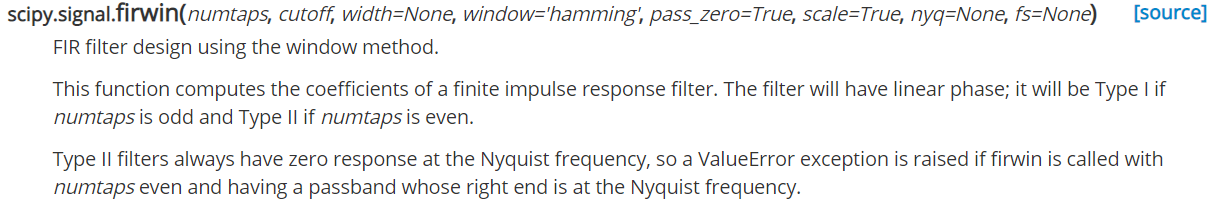
\includegraphics[width=\textwidth]{firwin.png}
    \caption{Function prototype and description for \texttt{firwin}.}
    \label{fig:firwin}
\end{figure}

\subsection{Optimal FIR Filter}
Digital filters designed via the window method have the largest ripples at the passband and stopband edges. The optimal method of FIR filter design aims to keep the ripple
constant in the passbands and stopbands. FIR filter coefficients are calculated by this method with the SciPy function remez, which is described in Fig. 2. For the same
reason described in Section 2.1, \texttt{numtaps} passed to \texttt{remez} was 399. The sampling frequency fs was 1024 Hz.\\

\noindent Ideally, the notch filters would attenuate only the additive noise frequencies, while not affecting frequencies. Zooming in on the ECG spectrum showed that
the noise existed almost entirely in the bands 32.5 – 32.7 Hz and 61.6 – 61.8 Hz; these frequencies define the stopband edges. To define the \texttt{bands} parameter, it is
also necessary to choose a transition bandwidth. Reducing the transition bandwidth results in less stop-band attenuation. By experimentation, it was found that a transition
bandwidth of 3.5 Hz eliminated the noise frequencies. The bands parameter was passed as $[0, 29, 32.5, 32.7, 36.2, 58.1, 61.6, 61.8, 65.3, 512]$. The desired gain in each
band of \texttt{bands} is defined by \texttt{desired}, which must be half the length of bands. The value for desired $[1, 0, 1, 0, 1]$.

\begin{figure}[H]
    \centering
    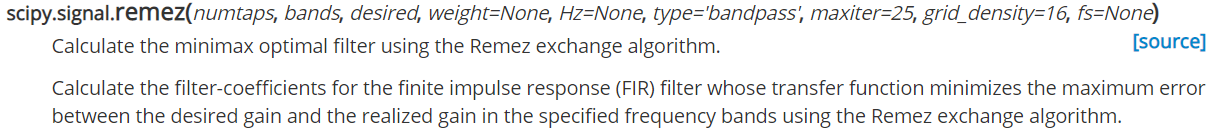
\includegraphics[width=\textwidth]{remez.png}
    \caption{Function prototype and description for \texttt{remez}.}
    \label{fig:remez}
\end{figure}

\subsection{Frequency Sampled FIR Filter}
ciPy does not define a function to design a frequency-sampled FIR filter, so a Python script was written to do this. The script was adapted from an example found in [2].
The script takes 400 equally spaced samples of the ideal frequency response with one sample taken at 0 Hz (i.e. a type 1 sampling scheme). Two transition samples were used,
though this can easily be changed with the \texttt{num\_transition\_samples} variable. The transition samples are equally spaced in magnitude, though ideal magnitude spacing may be
derived by extending the work in [3]. The inverse discrete Fourier transform of the ideal frequency response is calculated, giving the impulse response, which is then
shifted to make it symmetrical. The symmetrical impulse response is then tapered by a Hamming window.

\subsection{Pole-Zero Placed IIR Filters}
A simple method for IIR filter design is pole-zero placement on the z-plane. Zeros are placed in locations where the desired frequency response is zero. Poles are placed at
the same angle as the poles; their radii determine the transition bandwidth. To keep filter coefficients real, complex poles and zeros must come in complex-conjugate pairs.\\

\noindent For a notch filter, the angles the angle to place zeros (and poles) are:
\begin{equation}
    \textrm{arg}(z) = \pm \ang{360} \frac{f_{\textrm{notch}}}{f_s}
\end{equation}

\noindent With noise frequencies at 32.6 Hz and 61.7 Hz, zeros and poles were placed at ±11.46° for one notch filter and ±21.69° for the other notch filter. The 3 dB bandwidth of the
filters was specified as f3dB = 5 Hz, and the pole radius was calculated with:
\begin{equation}
    r = 1 - \frac{BW}{f_s}\pi
\end{equation}

\noindent Giving $r = 0.9847$ for both filters. To remove both noise frequencies, the IIR filters were cascaded together. Scaling factors of $0.99057$ and $0.98633$ were calculated and applied to
maintain unity passband gain. Figure 3 shows the final filter realisation.

\begin{figure}[H]
    \centering
    \begin{circuitikz}[american]
    \draw (0,0) node[draw,circle,minimum size=10pt]{+};
    \draw (2,0) ++(0.5,0) node[buffer](buffzero){\tiny 0.9906};
    % \draw (buffzero.out) -- node[draw,circle,minimum size=10pt]{+};
\end{circuitikz}
    \caption{Realisation of the cascaded IIR notch filters.}
    \label{fig:iir-filt}
\end{figure}
\section{Results}

\subsection{Noisy ECG Signal and Spectrum}

\subsection{Window FIR Filter}

\subsection{Optimal FIR Filter}

\subsection{Frequency Sampled FIR Filter}

\subsection{Cascaded Pole-Zero Placed IIR Filters}

\subsection{Noise Power Estimate}

\section{Discussion}

\section{Conclusion}

\section*{References}
\end{document}